\documentclass[a4paper, 12pt, oneside]{scrbook}
\usepackage[style=authoryear,backend=biber]{biblatex}
%Farbige Tabelle
\usepackage[table,dvipsnames]{xcolor}
%\addbibresource{bibliography.bib}
\usepackage[ngerman]{babel}		
%=====Schrift============================
%\usepackage{helvet}
\usepackage{mathptmx} 
\renewcommand{\familydefault}{\rmdefault} 
%-----
\usepackage[T1]{fontenc}
\usepackage[utf8]{inputenc}
\usepackage{graphicx}
\usepackage{epstopdf}
\usepackage{float}
\usepackage{acronym}
\usepackage{booktabs}
\usepackage{caption}
\usepackage{csquotes}
\usepackage{fancyhdr}
\usepackage{url}
\usepackage{listings} 
\usepackage[datesep=.]{datetime2}
\DTMsetstyle{ddmmyy}
\usepackage[binary-units=true]{siunitx}
%Enforce pictures to be in the same section. Use \FloatBarrier before a new subsection to enforce it on subsection level.
\usepackage[section]{placeins}
%Landscape support for pdfs.
\usepackage{pdflscape}
\usepackage[subfigure]{tocloft}

%Settings for the header line
\newcommand{\defineHeader}{
\pagestyle{fancy}
\lhead{}
\chead{}
\rhead{\rightmark}
\renewcommand{\headrulewidth}{1pt}}


%Do not reset footnote numbering
\usepackage{chngcntr}
\counterwithout{footnote}{chapter}

\renewcommand{\lstlistoflistings}{\begingroup
\tocfile{\lstlistingname}{lol}
\endgroup}

%Selbst eingefügte
%TimesNewRoman
\usepackage{mathptmx}
\usepackage{lipsum,mathptmx,etoolbox}% http://ctan.org/pkg/{lipsum,mathptmx,etoolbox}
\makeatletter
\usepackage{subfigure} 

%Zeilenabstand auf 1,5 gesetzt
\usepackage[onehalfspacing]{setspace}
\usepackage{wrapfig}
\usepackage{tocbibind}
\usepackage{pdfpages}
\usepackage{enumitem}
\definecolor{tecrmigreen}{HTML}{1EA12D}
\definecolor{tecallianceBlue}{HTML}{193366}
%Zum durchgehenden Numerieren der Abbildungen
\usepackage{chngcntr}
\counterwithout{figure}{chapter}
\counterwithout{table}{chapter}
%Um SubSubSection auch numeriert zu bekommen
%\setcounter{secnumdepth}{3}

\usepackage{multirow}
\usepackage[right]{eurosym} 
\usepackage{longtable}

\usepackage{blindtext}
%Load hyperref at the end, otherwise it could be that the footnotes are broken
\usepackage[hidelinks]{hyperref}

\renewcommand*{\headfont}{\normalfont}
\renewcommand*{\multicitedelim}{\addsemicolon\space}
\renewcommand*{\headrulewidth}{0pt}
\renewcommand*{\arraystretch}{1.5}

\setlength{\parskip}{1.5ex}
% Absätze am Seitenende müssen mindestens drei Zeilen haben
\clubpenalties=3 10000 7500 2500
\widowpenalties=3 10000 7500 2500


%Listing
\usepackage{color}
\definecolor{gray}{rgb}{0.4,0.4,0.4}
\definecolor{darkblue}{rgb}{0.0,0.0,0.6}
\definecolor{cyan}{rgb}{.0,0.6,0.6}

%Farben Layout
\definecolor{backgroundWhite}{rgb}{1,1,1}
\definecolor{classesCyan}{rgb}{0.05, 0.545, 0.545}
\definecolor{keywordBlue}{rgb}{0.13,0.13,1}
\definecolor{commentGreen}{rgb}{0,0.5,0}
\definecolor{stringRed}{rgb}{0.7,0.05,0.05}
\definecolor{red}{rgb}{255,0,0}
\definecolor{borderGray}{rgb}{0.87,0.88,0.89}
\definecolor{brandBlue}{rgb}{0.30,0.50,0.74}
\definecolor{attributePurple}{rgb}{0.5,0.0,1}

%Farben für logische Einheiten
\definecolor{logicalUnitsBlue}{RGB}{85, 85, 255}
%\definecolor{logicalUnitsGreen}{RGB}{90, 255, 90}
\definecolor{logicalUnitsGreen}{RGB}{60, 190, 60}
\definecolor{logicalUnitsOrange}{RGB}{255, 165, 0}
\definecolor{logicalUnitsPink}{RGB}{255, 192, 203}

\lstset{
	basicstyle=\ttfamily,
	columns=fullflexible,
	showstringspaces=false,
	commentstyle=\color{gray}\upshape,
	numbers=left,
	%Um eine durchgehende Numerierung bei Listings zu erhalten
	numberbychapter=false
}



%Für das Anhangsverzeichnis
\makeatletter
\newcommand*{\maintoc}{% Hauptinhaltsverzeichnis
  \begingroup
    \@fileswfalse% kein neues Verzeichnis öffnen
    \renewcommand*{\appendixattoc}{% Trennanweisung im Inhaltsverzeichnis
      \value{tocdepth}=-10000 % lokal tocdepth auf sehr kleinen Wert setzen
    }%
    \tableofcontents% Verzeichnis ausgeben
  \endgroup
}
\newcommand*{\appendixtoc}{% Anhangsinhaltsverzeichnis
  \begingroup
    \edef\@alltocdepth{\the\value{tocdepth}}% tocdepth merken
    \setcounter{tocdepth}{-10000}% Keine Verzeichniseinträge
    \renewcommand*{\contentsname}{% Verzeichnisname ändern
      Anhang}%
    \renewcommand*{\appendixattoc}{% Trennanweisung im Inhaltsverzeichnis
      \setcounter{tocdepth}{\@alltocdepth}% tocdepth wiederherstellen
    }%
    \tableofcontents% Verzeichnis ausgeben
    \setcounter{tocdepth}{\@alltocdepth}% tocdepth wiederherstellen
  \endgroup
}
\newcommand*{\appendixattoc}{% Trennanweisung im Inhaltsverzeichnis
}
\g@addto@macro\appendix{% \appendix erweitern
  \if@openright\cleardoublepage\else\clearpage\fi% Neue Seite
  \phantomsection
  \addcontentsline{toc}{chapter}{\appendixname}% Eintrag ins Hauptverzeichnis
  \addtocontents{toc}{\protect\appendixattoc}% Trennanweisung in die toc-Datei
}

\g@addto@macro\appendix{%
  %\pagenumbering{Roman}%
  \addtocontents{toc}{\protect\renewcommand*{\protect\@pnumwidth}{3.5em}}%Seitenzahlen im Anhangverzeichnis nicht über Seitenrand hinaus. Problem entstand durch die langen römischen Zahlen. Siehe auch: http://www.komascript.de/node/608
}

\makeatother
\usepackage[toc,automake]{glossaries}
% Formatiere Glossareinträge:
\renewcommand{\glstextformat}[1]{\textbf{\em #1}}
%\renewcommand{\glstextformat}[1]{\textbf{\color{blue}\em #1}}

\usepackage{longtable}
\definecolor{tecrmigreen}{HTML}{1EA12D}
\definecolor{tecallianceBlue}{HTML}{193366}


%Custom Settings
%C# SourceCode format settings for listings
%\setmonofont{Consolas} %to be used with XeLaTeX or LuaLaTeX
\definecolor{bluekeywords}{rgb}{0,0,1}
\definecolor{greencomments}{rgb}{0,0.5,0}
\definecolor{redstrings}{rgb}{0.64,0.08,0.08}
\definecolor{xmlcomments}{rgb}{0.5,0.5,0.5}
\definecolor{types}{rgb}{0.17,0.57,0.68}



\setlength{\parindent}{0em} 

\addbibresource{bibliography.bib}

\makeglossaries
\makeindex
\begin{document}


%Enable the header with headerline etc. Command is defined in the settings file.
\defineHeader

\begingroup
\renewcommand\cftchapafterpnum{\vskip -2pt}
\setlength{\cftbeforechapskip}{10pt}
\setcounter{tocdepth}{1}
\tableofcontents
\endgroup
\newpage

\listoffigures
%\newpage
%\listoftables
\renewcommand{\lstlistingname}{Listingverzeichnis}
\newpage
\lstlistoflistings
\renewcommand{\lstlistingname}{Listing}

\mainmatter

\chapter{Implementierungen in Python}

\section{Warum Python?}

\section{Verwendete Bibliotheken}

\section{Installationsanleitung}
\textcolor{red}{MATPLOTLIB, NUMPY + What is Pip? + Command}


\section{Aufbau des Python Projekts}

\chapter{Kategorisierung von Sequenzen}
\label{chp:categorization}
Im folgenden Kapitel wird die Implementierung der Skripte vorgestellt, die unterschiedliche Eigenschaften von Sequenzen berechnen und ausgeben.
Die erstellten Auswertungen basieren auf den in Kapitel~\ref{chp:procedure} vorgestellten Eigenschaften und Vorgehen.
\section{Kategorisierte Eigenschaften}
Folgende Eigenschaften werden für Sequenzen ermittelt:
\begin{description}
	\item[Balance] Die Balance ist ein Maß für die \enquote{Richtung} in die eine Sequenz ausgerichtet ist. Damit wird der Tendenz zu 0 oder 1 ein Wert zugeordnet. Die Balance kann Werte zwischen 0 und 1 annehmen. Die beiden Grenzen sind ebenfalls im Wertebereich vorhanden. Eine Sequenz mit einer Balance von 0.5 gilt als ausgeglichen, das bedeutet, dass die Sequenz so viele 0er wie 1er enthält.
	\item[Frequenz] Die Frequenz ist ein Maß für die Aktivität an Wertewechseln innerhalb einer Sequenz. Ein Wert gegen 0 entspricht einer sehr inaktiven Sequenz mit nur sehr wenigen bis keinen Wertewechsel. Ein Wert von 1 steht für eine hochfrequente Sequenz, in der sehr viel Wertewechsel stattfinden.
	\item[Sub-Sequenz] Die zu analysierenden Sequenzen werden anhand ihrer Länge in kleinere Sub-Sequenzen aufgeteilt, für die ebenfalls die Balance und Frequenz berechnet werden.
\end{description}

\subsection{Berechnung Balance}

\subsubsection{Vorgehen}
Die Balance wird nach folgender Formel berechnet:
\[
Balance = \frac{Anzahl\ Wert = 1}{Gesamtl\ddot{a}nge\ der\ Sequenz}
\]
Bei einer leeren Sequenz ist der Standardrückgabewert 0.
Der berechnete Wert entspricht der im Abschnitt~\ref{subsection:balance} vorgestellten Balance(1).
\subsubsection{Beispiel für eine ausgeglichene Sequenz}
Die folgende Sequenz mit einer Länge von 10000 Einträgen folgt der folgenden Vorschrift und ist in Abbildung~\ref{fig:example_balance_equal} abgebildet:
\[ a_{n} =
\begin{cases}
1       & \quad \text{für } n < 5000\\
0  		& \quad \text{für } n > 5000
\end{cases}
\]

\begin{figure}[H]
	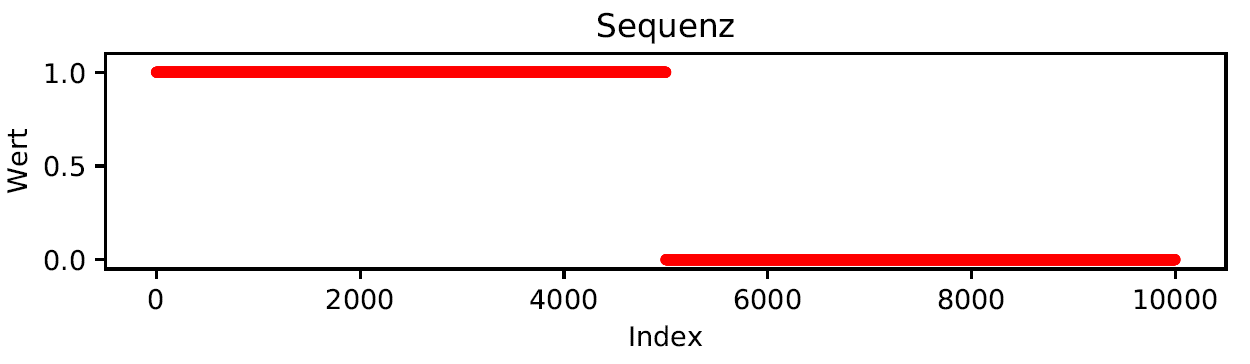
\includegraphics[width=\linewidth]{pythonImplementation/images/example_balance_equal.PNG}
	\caption[Darstellung einer ausgeglichenen Sequenz]{Stellt eine ausgeglichene (Balance = 0.5) Sequenz dar\footnotemark.}
	\label{fig:example_balance_equal}
\end{figure}
\footnotetext{ Quelle: Eigene Darstellung}

Für diese Sequenz wird eine Balance von 0.5 berechnet, da es genau so viele Werte mit 1 als auch 0 gibt. 
\subsubsection{Beispiel für eine unausgeglichene Sequenz}
Die folgende Sequenz mit einer Länge von 10000 Einträgen folgt der folgenden Vorschrift und ist in Abbildung~\ref{fig:example_balance_unequal} abgebildet:
\[ a_{n} =
\begin{cases}
1       & \quad \text{für } n < 9000\\
0  		& \quad \text{für } n > 1000
\end{cases}
\]

\begin{figure}[H]
	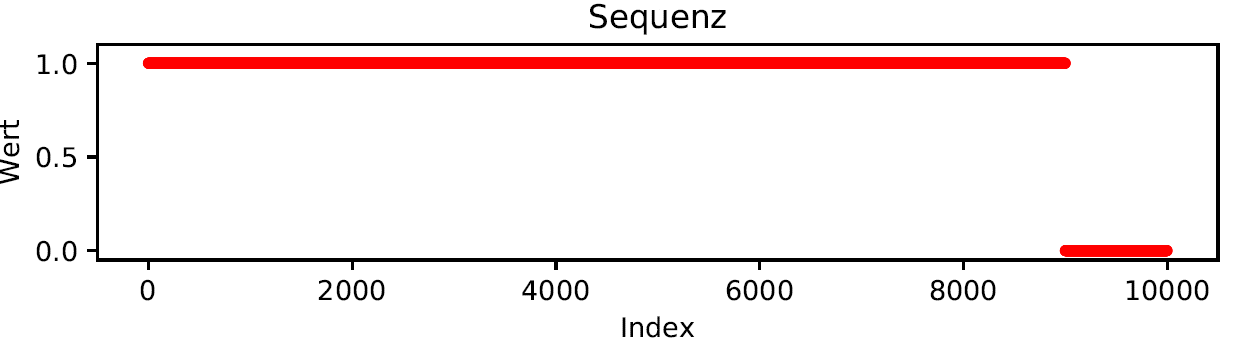
\includegraphics[width=\linewidth]{pythonImplementation/images/example_balance_unequal.PNG}
	\caption[Darstellung einer unausgeglichenen Sequenz]{Stellt eine unausgeglichene (Balance = 0.9) Sequenz dar\footnotemark.}
	\label{fig:example_balance_unequal}
\end{figure}
\footnotetext{ Quelle: Eigene Darstellung}

Für diese Sequenz wird eine Balance von 0.9 berechnet, da diese deutlich Richtung 1 tendiert. 
\subsection{Berechnung der Frequenz}

\subsubsection{Vorgehen}
Die Frequenz einer Sequenz wird nach folgender Formel berechnet:
\[
Frequenz = \frac{Anzahl\ der\ Wert\ddot{a}nderungen}{Gesamtl\ddot{a}nge\ der\ Sequenz}
\]

Ein Wert <= 0.25 gilt als \enquote{Niederfrequent}, ein Wert x > 0.25 und < 0.75 gilt als \enquote{Mittelfrequent} und Werte >= 0.75 als \enquote{Hochfrequent}.
Der Standardrückgabewert einer leeren Sequenz ist 0. 
Der berechnete Wert entspricht der im Abschnitt~\ref{subsection:frequence} vorgestellten Frequenz.

\subsubsection{Beispiel einer niederfrequenten Sequenz}
Eine niederfrequente Sequenz mit einer Länge von 10000 Einträgen ist in Abbildung~\ref{fig:example_frequence_low} abgebildet:

\begin{figure}[H]
	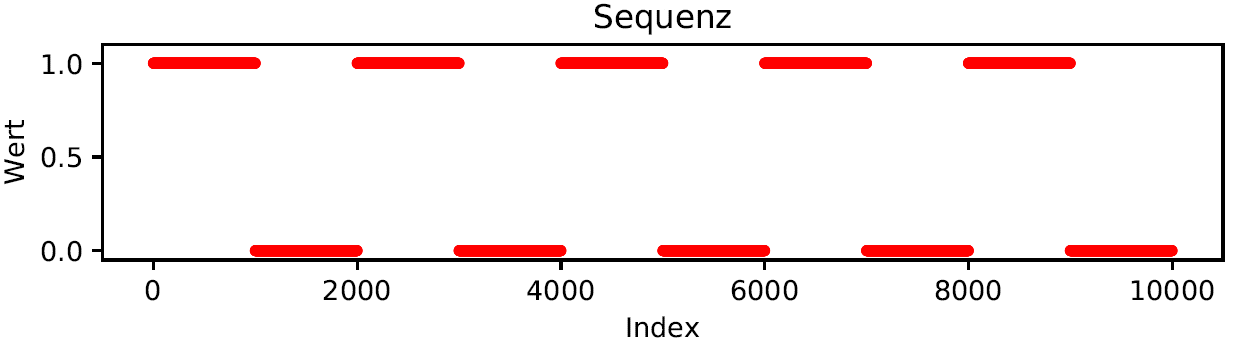
\includegraphics[width=\linewidth]{pythonImplementation/images/example_frequence_low.PNG}
	\caption[Darstellung einer niederfrequenten Sequenz]{Stellt eine niederfrequente Sequenz dar\footnotemark.}
	\label{fig:example_frequence_low}
\end{figure}
\footnotetext{ Quelle: Eigene Darstellung}

Diese Sequenz hat eine berechneten Frequenzwert von 0. Die Anzahl an Wertewechsel im Verhältnis zur Länge der Sequenz ist sehr niedrig.

\subsubsection{Beispiel einer mittelfrequenten Sequenz}
Eine mittelfrequente Sequenz mit einer Länge von 10000 Einträgen ist in Abbildung~\ref{fig:example_frequence_middle} abgebildet:

\begin{figure}[H]
	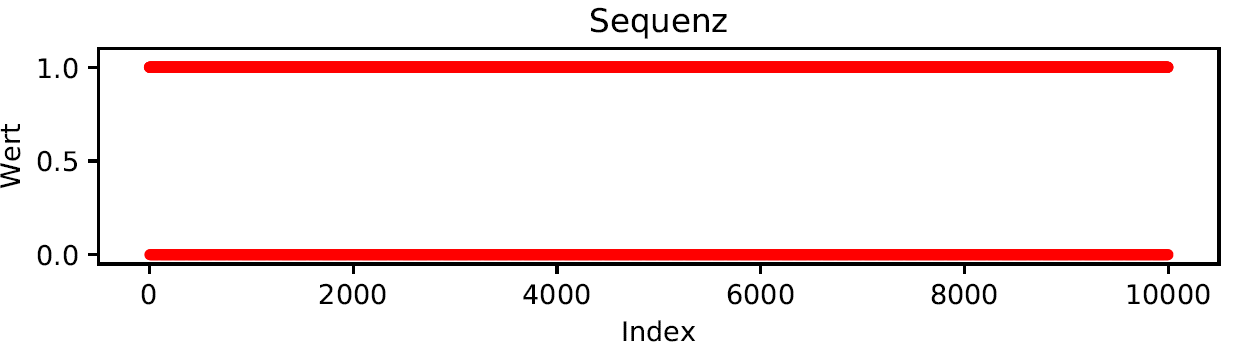
\includegraphics[width=\linewidth]{pythonImplementation/images/example_frequence_middle.PNG}
	\caption[Darstellung einer mittelfrequenten Sequenz]{Stellt eine mittelfrequente Sequenz dar\footnotemark.}
	\label{fig:example_frequence_middle}
\end{figure}
\footnotetext{ Quelle: Eigene Darstellung}

Diese Sequenz hat eine berechneten Frequenzwert von 0.4 und gilt damit als mittelfrequent.

\subsubsection{Beispiel einer hochfrequenten Sequenz}
Eine hochfrequente Sequenz mit einer Länge von 10000 Einträgen ist in Abbildung~\ref{fig:example_frequence_high} abgebildet:

\begin{figure}[H]
	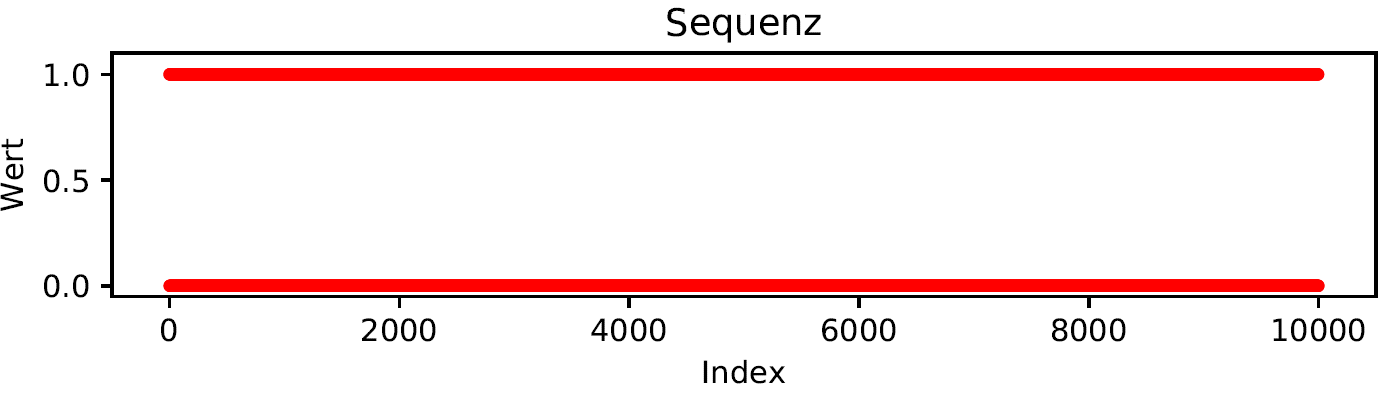
\includegraphics[width=\linewidth]{pythonImplementation/images/example_frequence_high.PNG}
	\caption[Darstellung einer hochfrequenten Sequenz]{Stellt eine hochfrequente Sequenz dar\footnotemark.}
	\label{fig:example_frequence_high}
\end{figure}
\footnotetext{ Quelle: Eigene Darstellung}

Diese Sequenz hat eine berechneten Frequenzwert von 0.9 und gilt damit als hochfrequent.

\subsection{Auswertung der Sub-Sequenzen}
Im Zuge des Projekts wurde ersichtlich, dass eine grafische Darstellung von Sequenzen in ihrer gesamten Länge nicht optimal für alle Fälle geeignet ist.
Wenn man die unterschiedlichen Sequenzen aus Abbildung~\ref{fig:example_frequence_middle} und Abbildung~\ref{fig:example_frequence_high} vergleicht, so sehen diese auf den ersten Blick identisch aus.
Bei der Auswertung der Frequenz sind diese aber unterschiedliche einzuordnen.
Dieser Effekt entsteht durch die Länge der Sequenzen und deren Darstellung in den generierten PDF Dateien.\\
Mit einer Analyse der Sequenzen in ihrer Gesamtlänge gehen auch zusätzliche Informationen verloren. Die Information ob eine Sequenz im ersten Drittel niederfrequent und zum Ende hin hochfrequent wird, kann durch einen einzelnen Zahlenwert nicht abgebildet werden.\\
Um die Unterschiede zu verdeutlichen, ist es notwendig die Sequenzen in kleinere Teilsequenzen zu unterteilen und diese zu vergleichen.\\
Die Aufteilung in Sequenzen entspricht dem in Kapitel~\ref{sec:classification} vorgestellten Vorgehen.

\subsubsection{Vorgehen zur Berechnung der Sub-Sequenzlängen}
Eine Sequenz wird je nach deren Länge in unterschiedlich große Teilsequenzen zerlegt. Diese Sub-Sequenzen werden ebenfalls im Bezug auf die Balance und Frequenz analysiert und die Ergebnisse werden in den entsprechenden PDF Dateien dargestellt.
Die Länge der Sub-Sequenzen wird dabei iterativ festgelegt. Das Vorgehen ist im Listing~\ref{lst:subSequenceLength} als Pseudo-Code dargestellt.\\

\lstnewenvironment{SubSequenceLength}
{\lstset{
		captionpos=b,
		frame=single,
		label={lst:subSequenceLength},
		caption={Pseudo-Code zur Festlegung der Länge der Sub-Sequenzen},
		showspaces=false,
		showtabs=false,
		breaklines=true,
		showstringspaces=false,
		breakatwhitespace=true,
		escapeinside={(*@}{@*)},
		commentstyle=\color{greencomments},
		morecomment = [l]{\#\ },
		morekeywords={ },
		keywordstyle=\color{blue},
		stringstyle=\color{black},
		morestring=[b]",
		basicstyle=\ttfamily\footnotesize,
		numberbychapter=false}}{}

\begin{SubSequenceLength}
int sequenceLength = length(sequence)
int subSequenceLength = 10

// Ensure there are at least 10 sub sequences:
while (sequenceLength / subSequenceLength ) >= 10
	SubSequenceLength is valid
	// Increase the size of the sub sequence by a factor of 10
	subSequenceLength = subSequenceLength  * 10
\end{SubSequenceLength}

Die Länge der möglichen Sub-Sequenzen startet bei 10 und wird bei jeder Iteration um den Faktor 10 erhöht. 
Dies geschieht so lange, bis die Anzahl der entstehenden Sub-Sequenzen 10 unterschreitet.\\
Eine Sequenz der Länge 1000 wird dabei in Sub-Sequenzen der Länge 10 und 100 aufgeteilt.
Eine Sequenz der Länge 10000 wird in Sub-Sequenzen der Länge 10, 100 und 1000 aufgeteilt.

\subsubsection{Benennung der Sub-Sequenzen}
In den Schaubildern und den generierten PDF-Dateien ist von 10er-Sub-Sequenzen, 100er Sub-Sequenzen usw. die Rede.
Die Zehnerpotenz ist dabei die Länge der Sub-Sequenz über die der Wert (Balance oder Frequenz) berechnet wurde.
Der Index auf der X-Achse entspricht dem Index der Sub-Sequenz.
Die erste 10er-Sub-Sequenz startet bei dem ersten Element in der Sequenz und beinhaltet die ersten 10 Elemente. 
Über diese Elemente wurden die Werte berechnet.
Die 10er-Sub-Sequenz mit dem nächst größeren Index enthält die nächsten 10 Elemente.
Die Sub-Sequenzen überschneiden sich dabei nicht.


\subsubsection{Beispiel für die analysierte Sub-Sequenzen}
Im Folgenden wird ein Beispiel für die generierten Sub-Sequenzen und deren Darstellung gegeben. 
Als Grundlage dient die in Abbildung~\ref{fig:example_subsequence} dargestellte Sequenz. 
Diese Sequenz hat eine Länge von 10000, ist mit einem Wert von 0.34 für die Frequenz mittelfrequent und gilt mit einem Balance-Wert von 0.17 als Unausgeglichen.
Man erkennt dass die Sequenz einige Intervalle mit einem Wert von 1 besitzt, wobei ein Wert von 0 klar dominiert.
Die Sequenz ist in dieser Form graphisch schwer zu analysieren, wenn man beispielsweise eine Aussage über die Länge der Ausschläge oder die Balance in Teilbereichen treffen will.

\begin{figure}[H]
	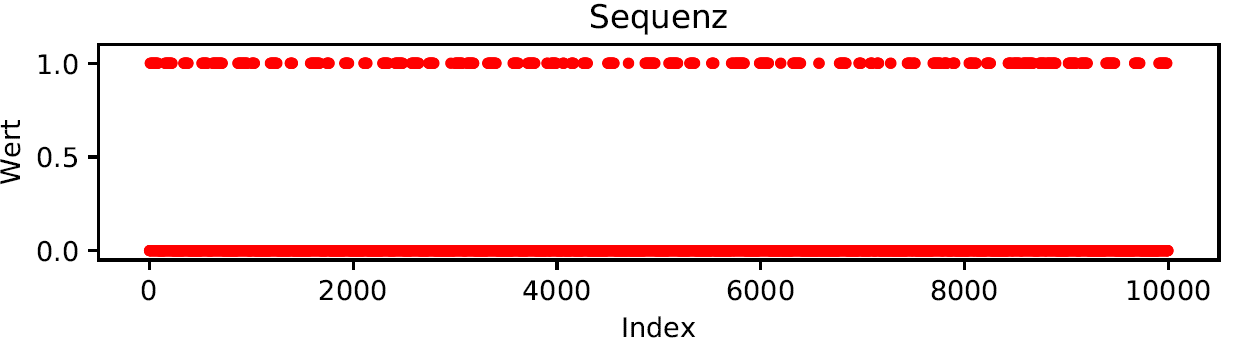
\includegraphics[width=\linewidth]{pythonImplementation/images/example_subsequences_main.PNG}
	\caption[Darstellung einer zu analysierenden Sequenz]{Stellt eine zu analysierende Sequenz dar\footnotemark.}
	\label{fig:example_subsequence}
\end{figure}
\footnotetext{ Quelle: Eigene Darstellung}

Stellt man allerdings die Teilsequenzen dar, erhöht sich der Detailgrad und es wird ein Verlauf der Frequenz und der Balance ersichtlich.
Durch den erhöhten Detailgrad können die Sequenzen besser analysiert werden (falls dies notwendig ist).
\\
In Abbildung~\ref{fig:example_subsequence_balances} ist die Balance der Sub-Sequenzen dargestellt.
In dieser Darstellung ist der Verlauf der Balance erkennbar, wodurch Intervalle mit gleicher Balance besser erkennbar sind.
Die unterschiedliche Länge der Sub-Sequenzen wirkt sich dabei auf die Darstellung aus.
Je größer die Sub-Sequenz ist, desto gleichmäßiger ist die Balance.
Dadurch sind gleichmäßige Intervalle in größeren Sub-Sequenzlängen besser erkennbar als in kleinen Längen.
Kurze Ausschläge sind allerdings in kurzen Sub-Sequenzlängen besser erkennbar.

\begin{figure}[H]
	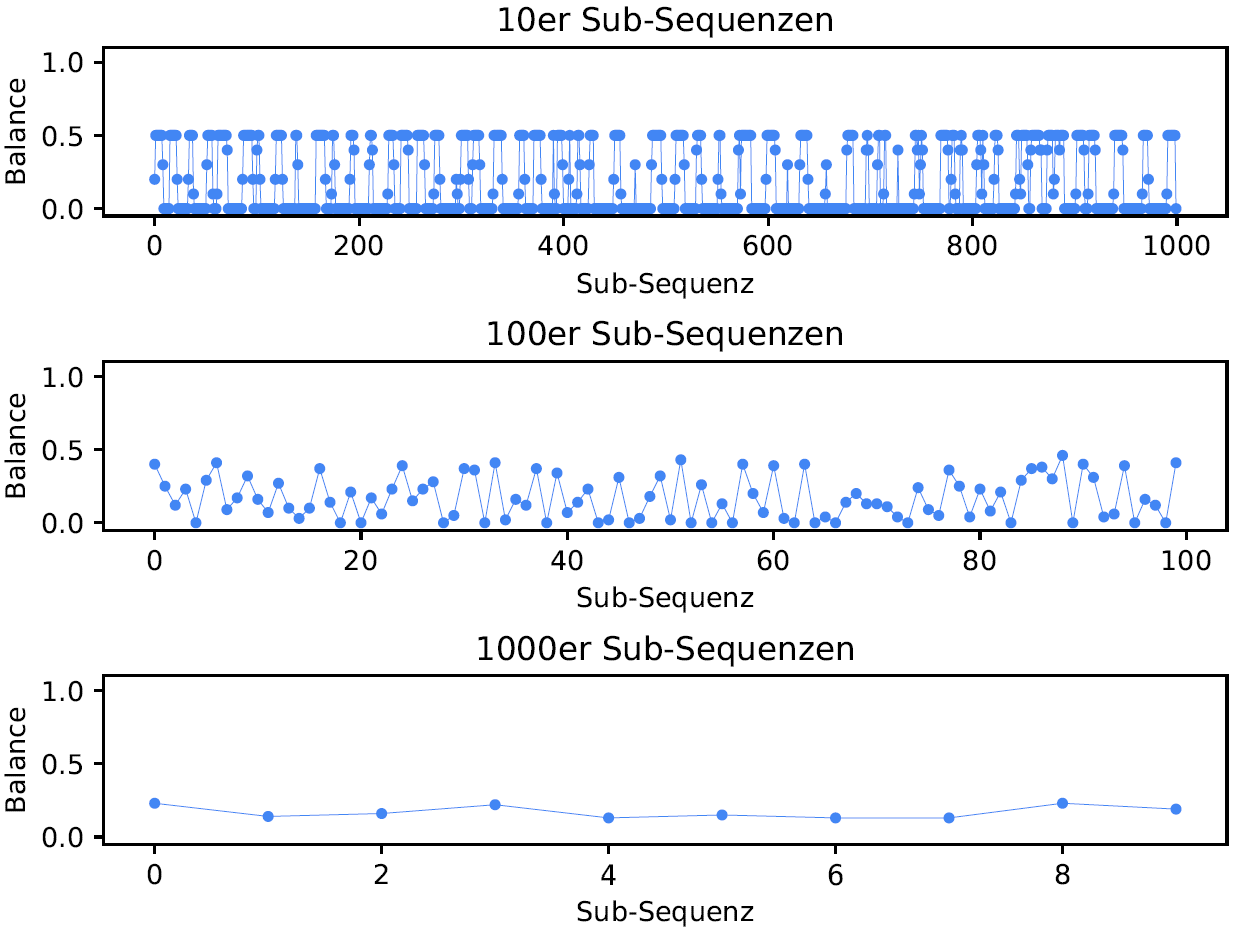
\includegraphics[width=\linewidth]{pythonImplementation/images/example_subsequences_balances.PNG}
	\caption[Darstellung der Sub-Sequenzen im Bezug auf die Balance]{Stellt die Balance der Sub-Sequenzen dar\footnotemark.}
	\label{fig:example_subsequence_balances}
\end{figure}
\footnotetext{ Quelle: Eigene Darstellung}

\newpage
Analog dazu wird auch die Frequenz der Sub-Sequenzen analysiert. Das Ergebnis ist in Abbildung~\ref{fig:example_subsequence_frequences} dargestellt.

\begin{figure}[H]
	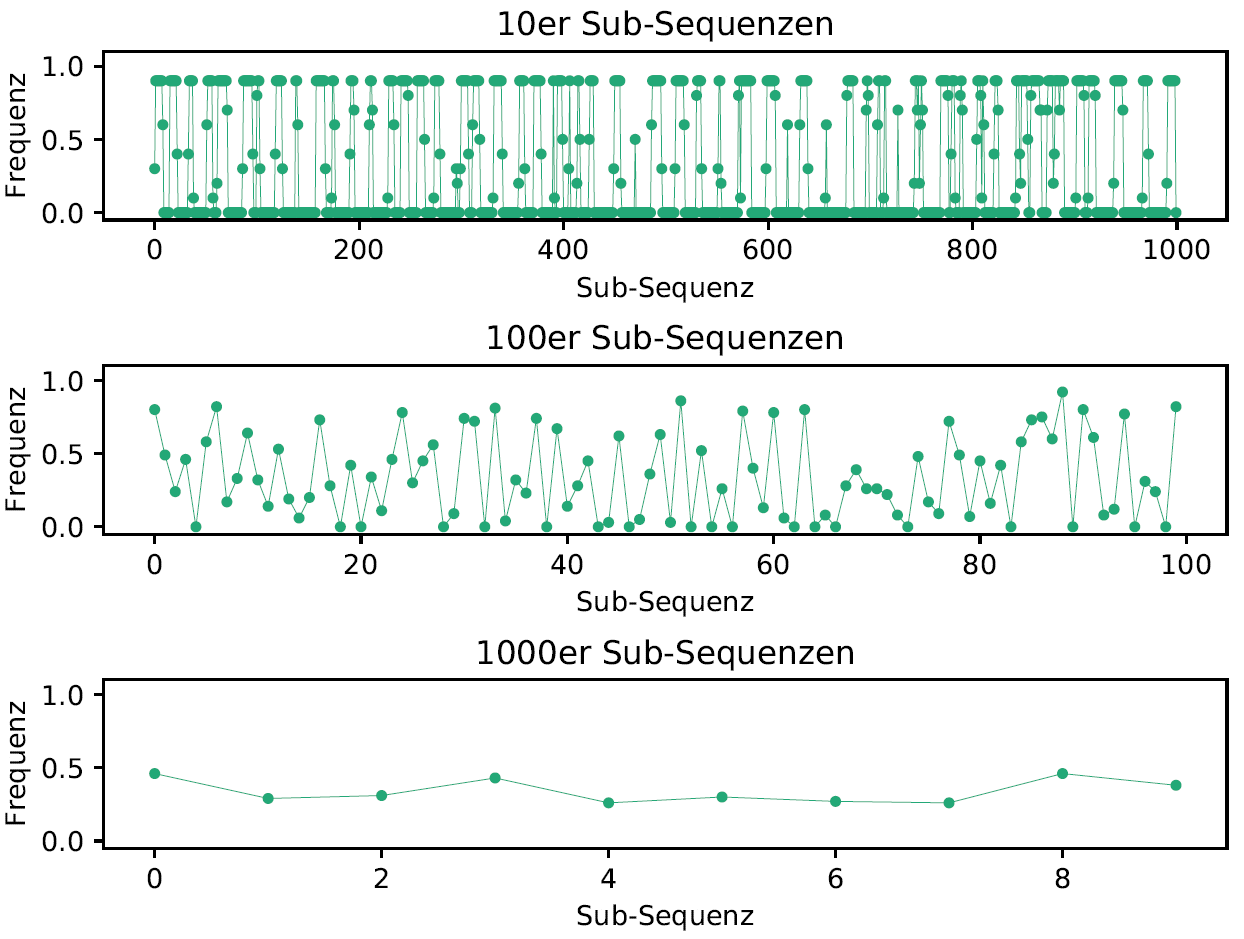
\includegraphics[width=\linewidth]{pythonImplementation/images/example_subsequences_frequences.PNG}
	\caption[Darstellung der Sub-Sequenzen im Bezug auf die Frequenz]{Stellt die Frequenz der Sub-Sequenzen dar\footnotemark.}
	\label{fig:example_subsequence_frequences}
\end{figure}
\footnotetext{ Quelle: Eigene Darstellung}



\subsubsection{Vergleich über die Sub-Sequenzen}
Über die Sub-Sequenzen können die Sequenzen in manchen Fällen besser verglichen werden.
Die in Abbildung~\ref{fig:example_frequence_middle} und Abbildung~\ref{fig:example_frequence_high} dargestellten Sequenzen sehen auf den ersten Blick identisch aus.
Allerdings unterscheiden sich diese in ihrem Wert für die Frequenz (0.4 zu 0.9).
Dieser Unterschied ist auch deutlich, wenn man sich die Frequenz der entsprechenden Sub-Sequenzen anschaut.\\
Die Sub-Sequenzen der mittelfrequenten Sequenz aus Abbildung~\ref{fig:example_frequence_middle} sind in Abbildung~\ref{fig:example_frequence_middle_subsequences} dargestellt. 
Es ist nicht überraschen, dass diese sehr konstant ist und den Frequenzwert von 0.4 wiedergibt.
\begin{figure}[H]
	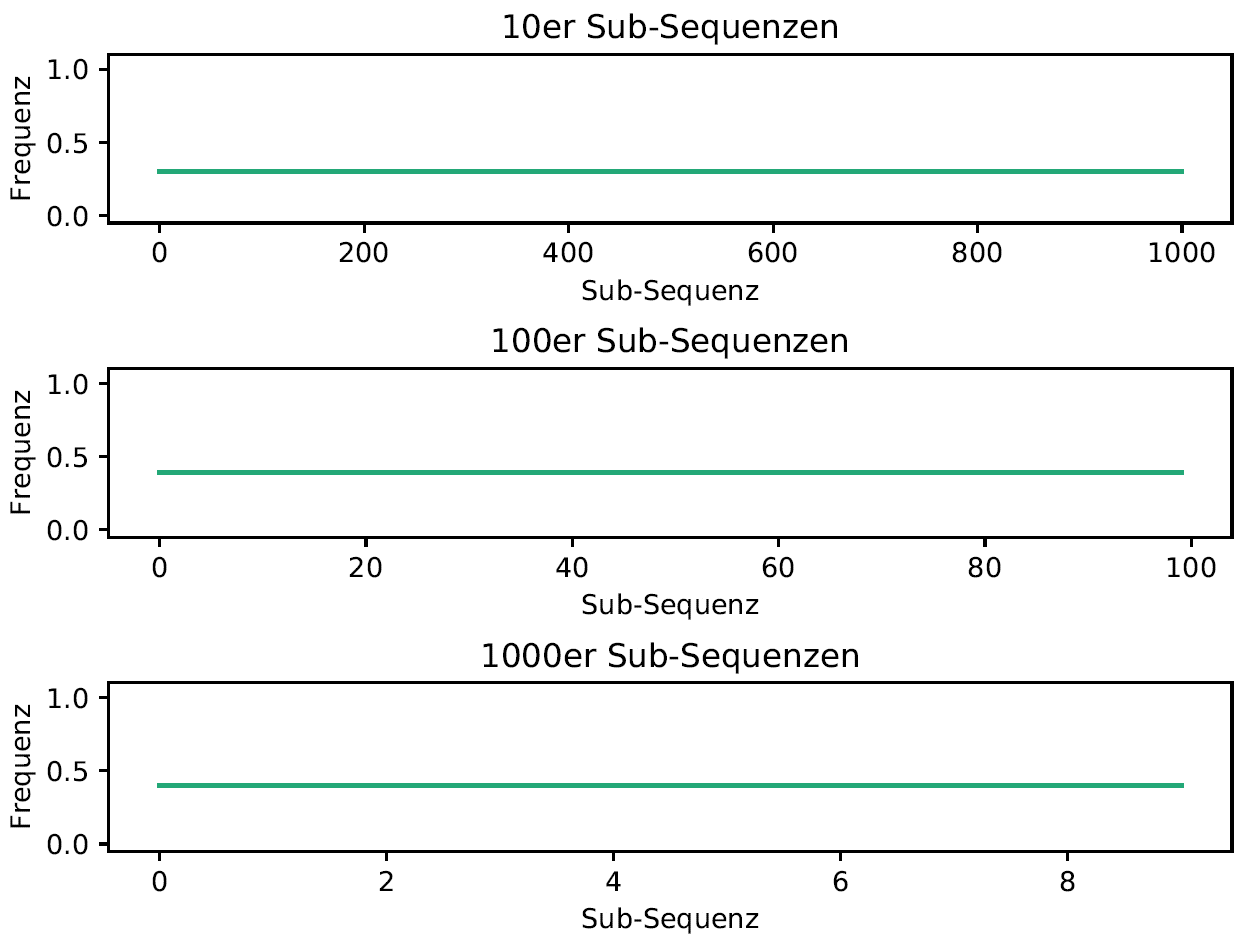
\includegraphics[width=\linewidth]{pythonImplementation/images/example_frequence_middle_subsequences.PNG}
	\caption[Darstellung der Sub-Sequenzen im Bezug auf die Frequenz einer mittelfrequenten Sequenz]{Stellt die Frequenz der Sub-Sequenzen einer mittelfrequenten Sequenz dar\footnotemark.}
	\label{fig:example_frequence_middle_subsequences}
\end{figure}
\footnotetext{ Quelle: Eigene Darstellung}

Die Sub-Sequenzen der hochfrequenten Sequenz aus Abbildung~\ref{fig:example_frequence_high} zeigen hingegen ein neues Detail, welches nicht in der Gesamtansicht erkennbar ist.
Auch hier ist der hohe Wert für die Frequenz erkennbar, allerdings ist dieser nicht so gleichmäßig wie bei der mittelfrequenten Sequenz.
Es gibt einzelne Spitzen, die über die gesamte Länge der Sequenz verteilt sind. 
Die Sub-Sequenzen sind in Abbildung~\ref{fig:example_frequence_high_subsequences} dargestellt.
\begin{figure}[H]
	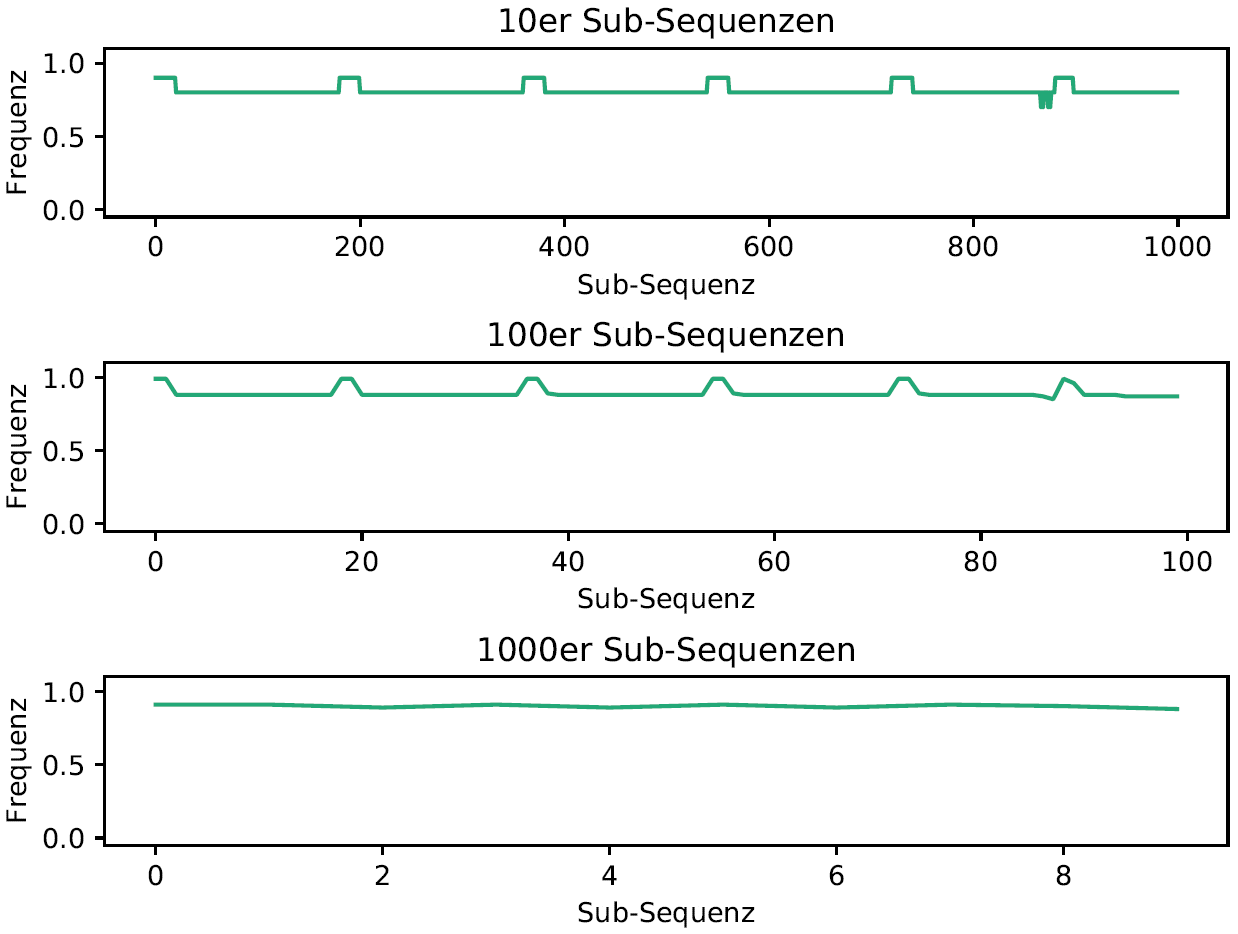
\includegraphics[width=\linewidth]{pythonImplementation/images/example_frequence_high_subsequences.PNG}
	\caption[Darstellung der Sub-Sequenzen im Bezug auf die Frequenz einer hochfrequenten Sequenz]{Stellt die Frequenz der Sub-Sequenzen einer hochfrequenten Sequenz dar\footnotemark.}
	\label{fig:example_frequence_high_subsequences}
\end{figure}
\footnotetext{ Quelle: Eigene Darstellung}

\chapter{Kreuzkorrelation und Faltung}
\section{Einführung Kreuzkorrelation}
Die Kreuzkorrelation wird verwendet, um die Korrelation zwischen zwei Signalen oder Sequenzen zu berechnen. Dabei werden unterschiedliche Zeitverschiebungen zwischen
den Sequenzen eingesetzt. NumPy verwendet dabei folgende Formel für die 
Kreuzkorrelation\footnote{Siehe: Dokumentation NumPy:\cite{DocumentationNumpyCorrelate} und Definition Kreuzkorrelation: \cite{DefinitionCrossCorrelation}.}.

\[
  f \star g \equiv \int\limits_{-\infty}^{+\infty} \overline{f}(-t)*g(t)
\]
Die Formel kann in eine Form umgewandelt werden, aus der die Verschiebung einer Sequenz gegenüber einer anderen besser ersichtlich 
ist\footnote{Umformung: siehe: \cite{DefinitionCrossCorrelation}.}:
\[
  f \star g \equiv \int\limits_{-\infty}^{+\infty} \overline{f}(-\tau)*g(t + \tau) \text{ } \mathrm{d}\tau
\]

NumPy bietet dabei unterschiedliche Modi bei der Berechnung der Kreuzkorrelation an. Diese entsprechen den Modi der mathematischen Faltung ( zu Englisch \enquote{Convolution}).
Die Unterschiede der Kreuzkorrelation und Faltung sowie der Autokorrelation sind in den folgenden Abbildungen dargestellt.
Abbildung~\ref{fig:compareConvulationCrosscorrelationAutoCorrelation} bietet einen Überblick, während die Abbildungen~\ref{fig:convolutionExample1} und \ref{fig:convolutionExample2} animiert sind.
Sollte die Animation nicht korrekt dargestellt werden, sind diese über die jeweilige Quellenangaben einsehbar.

\section{Beispiele Kreuzkorrelation, Faltung und Autokorrelation}
\begin{figure}[H]
  \centering
  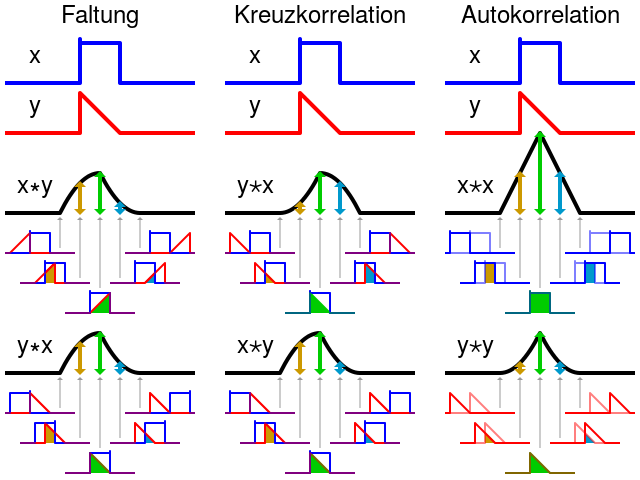
\includegraphics[width=0.8\linewidth]{./images/comparisonConvolutionCorrelation.png}
  \caption[Vergleich zwischen Faltung, Kreuzkorrelation und Autokorrelation]{Vergleicht die Faltung, Kreuzkorrelation und Autokorrelation\footnotemark}
  \label{fig:compareConvulationCrosscorrelationAutoCorrelation}
\end{figure}
\footnotetext{Quelle: \cite[]{CompareConvulationCrosscorrelationAutoCorrelation}}

\begin{figure}[H]
  \centering
  \animategraphics[loop,autoplay,label=convolutionExample1]{25}{./images/convolutionExample1/frame_}{1}{301}
  \caption[Animation: Beispiel 1 für die Faltung]{Darstellung einer eindimensionalen Faltung\footnotemark}
  \label{fig:convolutionExample1}
\end{figure}
\footnotetext{Quelle: \cite[]{ConvultionExample1Wikimedia}}

\begin{figure}[H]
  \centering
  \animategraphics[loop,autoplay]{25}{./images/convolutionExample2/frame_}{1}{161}
  \caption[Animation: Beispiel 2 für die Faltung]{Faltung zweier Gaussfunktionen\footnotemark}
  \label{fig:convolutionExample2}
\end{figure}
\footnotetext{Quelle: \cite[]{ConvultionExample2Wikimedia}}

\section{Bedeutung der unterschiedlichen Modi}
\begin{samepage}
  In den Beschreibungen gelten folgende Voraussetzungen: 
  \begin{align*}
    & \text{Sequenz A: von }a[0] \text{ bis }a[L_A - 1] \text{ mit } L_A = \text{Länge von Sequenz A}\\
    & \text{Sequenz A: von }b[0] \text{ bis }b[L_B - 1] \text{ mit } L_B = \text{Länge von Sequenz B}
  \end{align*}
  Als Quelle dient die Dokumentation\footnote{Dokumentation NumPy Correlate: \cite{DocumentationNumpyCorrelate}.} sowie eine Beschreibung der 
  Modi\footnote{Beschreibung der Modi: \cite{NumPyCorrelationModesExplained}.}.
\end{samepage}


\subsection{Modus: Valid}
Dieser Modus wird verwendet, wenn der Modus nicht explizit angegeben wird.\\
Dabei wird eine Ausgabe der Länge $ max(L_A, L_B) - min(L_A, L_B) + 1 $ erzeugt. Die Verschiebung findet dabei im Bereich 
von $ min(L_A, L_B) - 1 \text{ bis } - max(L_A, L_B) - 1 $ statt.

\subsection{Modus: Full}
In diesem Modus wird die Berechnung im Bereich von $ 0 \text{ bis }  L_A + L_B - 2 $ durchgeführt. 
Dadurch ergibt sich eine Ausgabe von $ L_A + L_B + 1 $ Elementen. Dabei können Effekte an den Rändern der Sequenzen auftreten, da diese
sich dort nicht mehr voll überlappen.

\subsection{Modus: Same}
Liefert ein Ergebnis der Länge $ max(L_A, L_B) $ . Dabei können ebenfalls Effekte an den Rändern auftreten.\\
Die Berechnug findet im Bereich von $ \frac{(L_B - 1)}{2} \text{ bis } L_A - 1 + \frac{L_B - 1}{2} $ statt. \\
Sollte $ L_A < L_B $ gelten, werden die beiden Sequenzen vor der Berechnung ausgetauscht.











\chapter{Funktion zur Berechnung der Kreuz-Korrelation}
Die Skripte zur Berechnung der Kreuz-Korrelation befinden sich im \enquote{crosscorrelation}-Verzeichnis.
Das Python Skript \enquote{functions\_crosscorrelation.py} bietet als Einstiegspunkt die Funktion\\ \mbox{\enquote{crossCorrelation(...)}} an. Im Folgenden werden die Parameter und deren Bedeutung beschrieben.

\section{Beschreibung der Parameter}

Es gibt drei Parameter, die beim Aufruf der Funktion mitgegeben werden müssen. Dabei handelt es sich um die beiden Sequenzen, die verarbeitet werden sollen sowie um die Einstellungen. Aufgrund der vielen Einstellungsmöglichkeiten, wurden diese in eigene eigene Klasse ausgelagert, die beim Aufruf als dritter Parameter übergeben werden muss.
\begin{description}[style=nextline]
\item[seqA] Die erste Datensequenz in Form eines eindimensionalen Arrays. Die enthaltenen Zahlenwerte müssen in Float konvertierbar sein.
\item[seqB] Die zweite Datensequenz in Form eines eindimensionalen Arrays. Die enthaltenen Zahlenwerte müssen in Float konvertierbar sein.
\end{description}

\subsection{Einstellungsparameter}
Folgende Parameter stehen für die Konfiguration zur Verfügung. Die standardmäßig gesetzten Werte sind mit angegeben:
\begin{description}[style=nextline]
\item[plotNormalizedData] [Default: False] Auf True setzen, wenn die beiden Sequenzen auch normalisiert dargestellt werden sollen.
\item[plotCorrelations] [Default: False] Auf True setzen, wenn die berechnete Kreuz-Korrelation dargestellt werden soll. Dabei werden alle drei Berechnungsmethoden \enquote{Valid}, \enquote{Same} und \enquote{Full} dargestellt.
\item[plotNonNormalizedResults] [Default: False] Auf True setzen, wenn auch die unnormalisierten Ergebnisse dargestellt werden sollen.
\item[plotNormalizedResults] [Default: True] Auf False setzen, wenn auch die normalisierten Ergebnisse nicht dargestellt werden sollen.
\item[subtractMeanFromResult] [Default: True] Auf False setzen, wenn das arithmethische Mittel nicht von den Ergebnissen abgezogen werden soll.
\item[drawResults] [Default: False] Wird dieser Parameter auf True gesetzt, werden die Ergebnisse auf dem Bildschirm ausgegeben. Dies kann sinnvoll sein, wenn keine PDF-Dateien erstellt werden sollen, die Ergebnisse aber dennoch sichtbar sein sollten. Der Standardwert ist auf False gesetzt, da die Skripte automatisiert durch weitere Skripte aufgerufen werden. Die Verarbeitung der Skripte blockiert dabei solange das Fenster zur Anzeige geöffnet ist. In einem automatisierten Kontext würde niemand das Fenster schließen, wodurch der Prozess blockiert werden würde.
\item[exportToPdf] [Default: False] Auf True setzen, wenn eine PDF-Datei mit den Ergebnissen generiert werden soll.
\item[exportFilePath] [Default: \enquote{}] Der Pfad zur PDF-Datei, in dem die Ergebnisse gespeichert werden sollen. Wenn \enquote{exportToPdf} auf True gesetzt wird, muss mit dieser Einstellung der Pfad zur PDF-Datei angegeben werden. Ansonsten wird die Einstellung ignoriert.
\end{description}

\section{Beispiel Ergebnisse}
Es gilt für alle Beispiele (solange nicht im Beispiel genauer spezifiziert):\\
Vorbedingung: Zwei Sequenzen mit je 10000 Einträgen. \\
SeqA:
\[ a_{n} =
  \begin{cases}
    1       & \quad \text{wenn } n \text{ enthalten in [1005,2005,1505,3505,5505,6005,6505,8005,8505,9005]}\\
    0  & \quad \text{sonst}
  \end{cases}
\]
SeqB:
\[ b_{n} =
  \begin{cases}
    1       & \quad \text{wenn } n \text{ enthalten in [1000,2000,1500,3500,5500,6000,6500,8000,8500,9000]}\\
    0  & \quad \text{sonst}
  \end{cases}
\]
Es ist ersichlich, dass die Sequenzen zueinander um einen Index von 5 verschoben sind.

\subsection{Anzeige der beiden Sequenzen mit normalisiertem Ergebnis}
Der Aufruf der Funktion mit den Standard-Parametern der Einstellungen, liefert für die Beispielsequenzen folgendes Ergebnis (dargestellt in Abbildung~\ref{fig:correlationDefaultParams}):
\begin{figure}[H]
    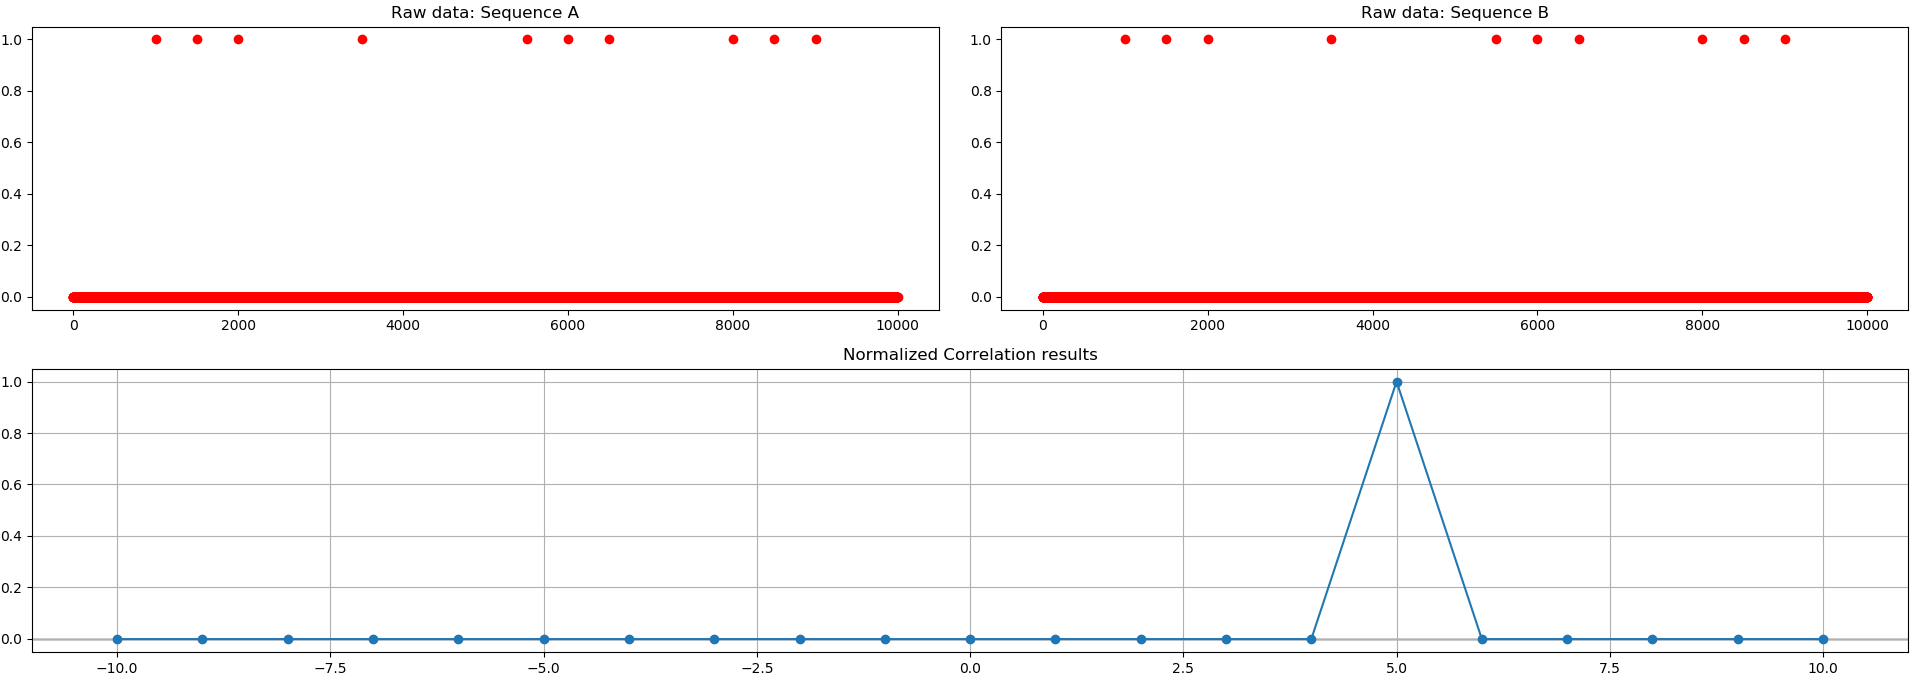
\includegraphics[width=\linewidth]{pythonImplementation/images/correlationDefaultParams.PNG}
    \caption[Ergebnis: Default-Parameter]{Ergebnis der Funktion bei Default-Parametern\footnotemark.}
    \label{fig:correlationDefaultParams}
\end{figure}
\footnotetext{Quelle: Eigene Darstellung}

\subsection{Auswirkungen des Parameter: plotNormalizedData}
Durch setzen des optionalen Parameters \enquote{plotNormalizedData} auf True, werden die beiden Sequenzen, zusätzlich in normalisierter Form dargestellt. 
Siehe dazu Abbildung~\ref{fig:correlationPlotNormalizedData}. 
\begin{figure}[H]
    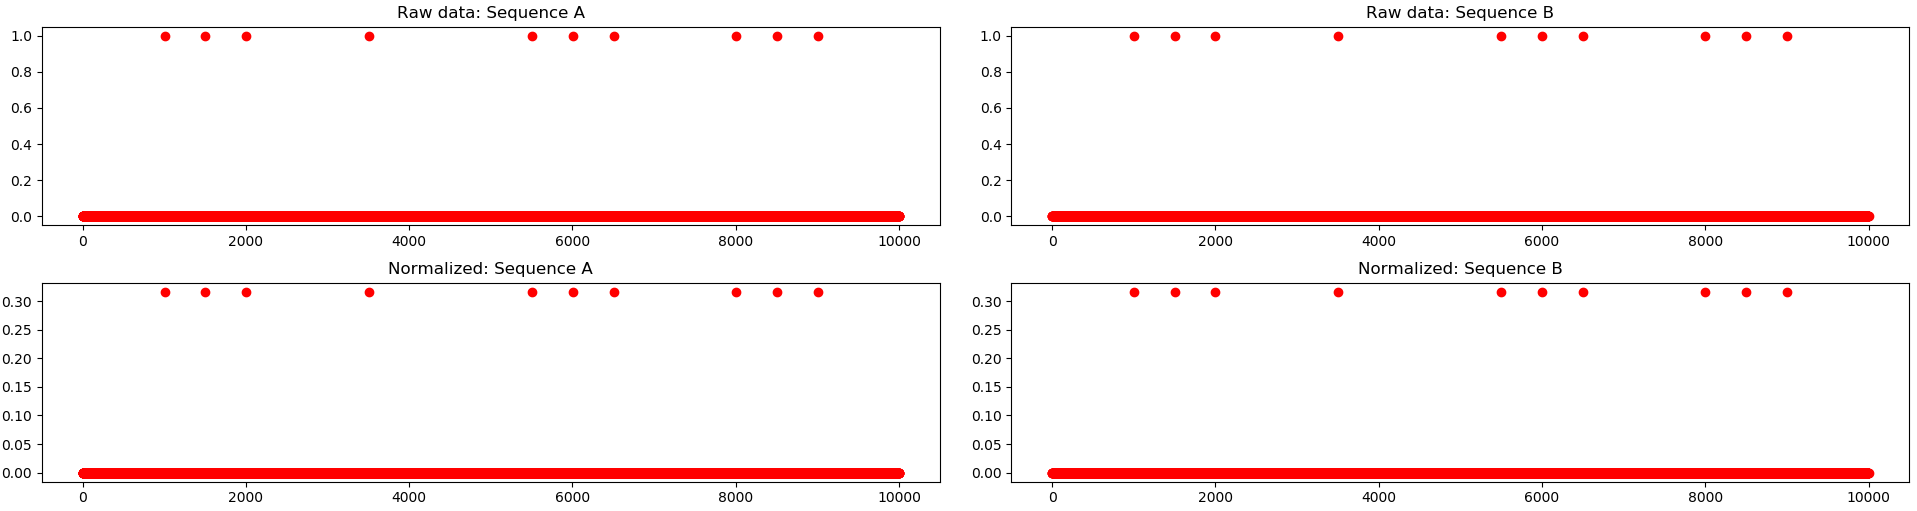
\includegraphics[width=\linewidth]{pythonImplementation/images/correlationPlotNormalizedData.PNG}
    \caption[Ergebnis: plotNormalizedData]{Ergebnis der Funktion bei \enquote{plotNormalizedData = True} (Darstellung der Ergebnisse weggelassen)\footnotemark. }
    \label{fig:correlationPlotNormalizedData}
\end{figure}
\footnotetext{Quelle: Eigene Darstellung}

\subsection{Auswirkungen des Parameter: plotCorrelations}
Durch setzen des optionalen Parameters \enquote{plotCorrelations} auf True, 
wird die Kreuz-Korrelation der beiden Sequenzen berechnet.
Dabei werden alle drei Berechnungsmethoden \enquote{Valid}, \enquote{Same} und \enquote{Full} dargestellt.
Siehe dazu Abbildung~\ref{fig:correlationPlotCorrelations}. 
\begin{figure}[H]
    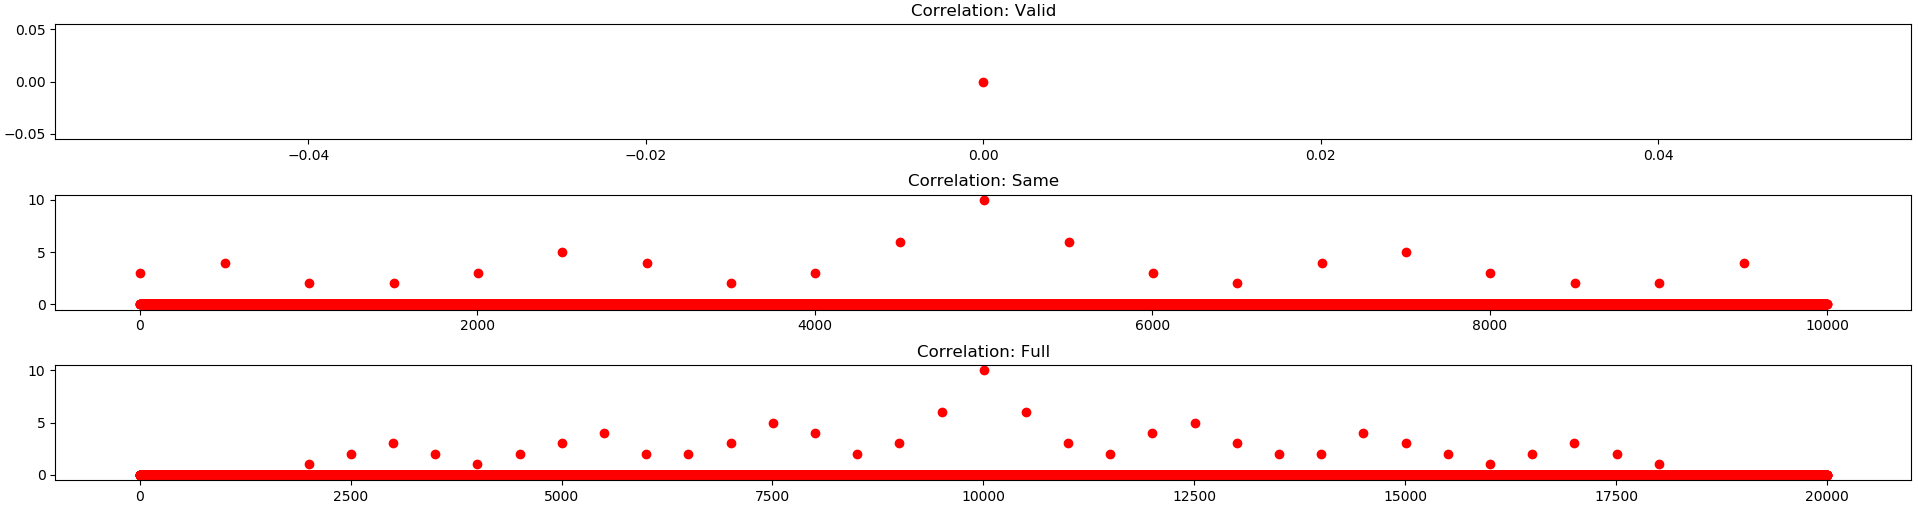
\includegraphics[width=\linewidth]{pythonImplementation/images/correlationPlotCorrelations.PNG}
    \caption[Ergebnis: plotCorrelations]{Zusätzliche Ausgabe der Funktion bei \enquote{plotCorrelations = True} (Darstellung der Ergebnisse weggelassen)\footnotemark. }
    \label{fig:correlationPlotCorrelations}
\end{figure}
\footnotetext{Quelle: Eigene Darstellung}

\subsection{Auswirkungen des Parameter: plotNonNormalizedResults}
Durch setzen des optionalen Parameters \enquote{plotNonNormalizedResults} auf True, können die Ergebnisse zusätzlich in unnormalisierter Form ausgegeben werden.
Siehe dazu Abbildung~\ref{fig:correlationPlotNonNormalizedResults}. 
\begin{figure}[H]
    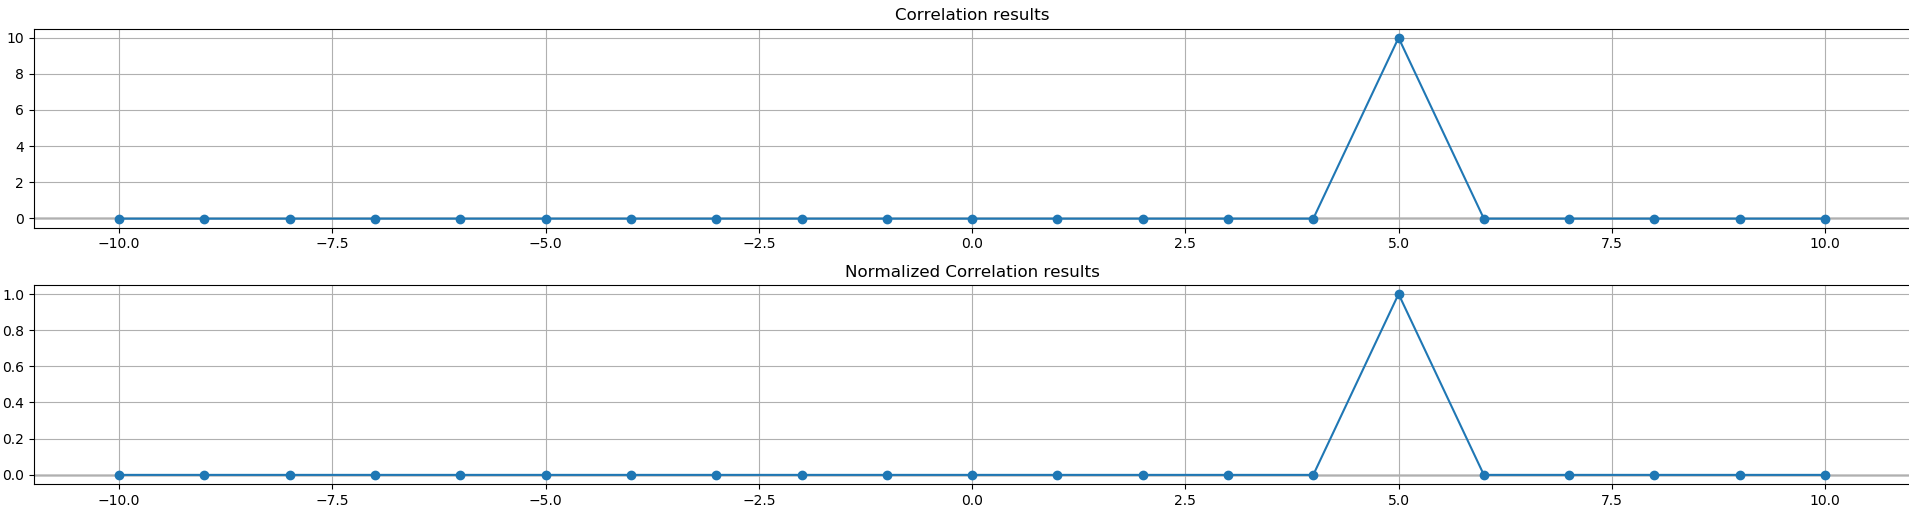
\includegraphics[width=\linewidth]{pythonImplementation/images/correlationPlotNonNormalizedResults.PNG}
    \caption[Ergebnis: plotNonNormalizedResults]{Zusätzliche Ausgabe der Funktion bei \enquote{plotNonNormalizedResults = True}\footnotemark. }
    \label{fig:correlationPlotNonNormalizedResults}
\end{figure}
\footnotetext{Quelle: Eigene Darstellung}

\subsection{Auswirkungen des Parameter: plotNormalizedResults}
Durch setzen des optionalen Parameters \enquote{plotNormalizedResults} auf False, kann die Ausgabe der normalisierten Ergebnisse verhindert werden.

\subsection{Auswirkungen des Parameter: subtractMeanFromResult}
Um die Auswirkung des Parameters darzustellen, werden folgende Sequenzen vorrausgesetzt (je 10000 Einträge):\\
SeqA:
\[ a_{n} =
  \begin{cases}
    2       & \quad \text{wenn } n \text{ enthalten in [1005,2005,1505,3505,5505,6005,6505,8005,8505,9005]}\\
    1  & \quad \text{sonst}
  \end{cases}
\]
SeqB:
\[ b_{n} =
  \begin{cases}
    2       & \quad \text{wenn } n \text{ enthalten in [1000,2000,1500,3500,5500,6000,6500,8000,8500,9000]}\\
    1  & \quad \text{sonst}
  \end{cases}
\]
Die Sequenzen sind wieder um einen Wert von 5 verschoben, allerdings wechseln diese nicht zwischen 0 und 1, sondern zwischen 1 und 2. 
Die Ergebnisse können dabei unübersichtlich werden, deshalb wird ohne Angabe des Parameters, True als Standardwert verwendet.
Dadurch wird das arithmethische Mittel des Ergebnis vom Ergebnis selbst abgezogen. Abbildung~\ref{fig:correlationSubtractMeamFromResultTrue} 
und \ref{fig:correlationSubtractMeamFromResultFalse} zeigen die Auswirkung des Parameters. 
\begin{figure}[H]
    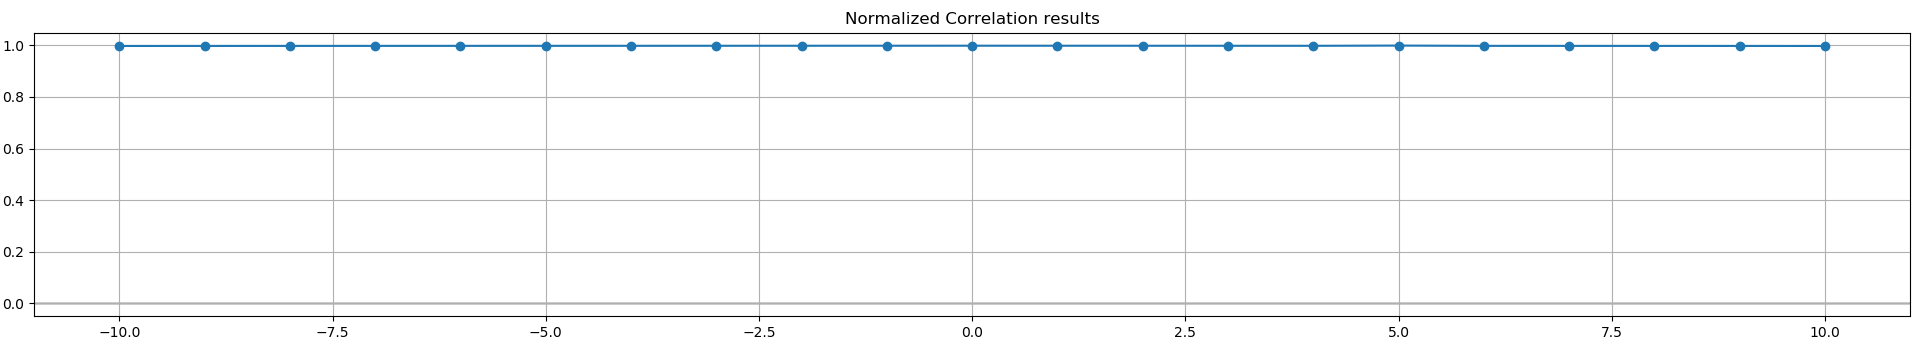
\includegraphics[width=\linewidth]{pythonImplementation/images/correlationSubtractMeamFromResultFalse.PNG}
    \caption[Ergebnis: subtractMeanFromResult = False]{Darstellung des Ergebnis bei \enquote{subtractMeanFromResult = False}. Ausschläge sind sehr schwer erkennbar\footnotemark. }
    \label{fig:correlationSubtractMeamFromResultFalse}
\end{figure}
\footnotetext{Quelle: Eigene Darstellung}

\begin{figure}[H]
    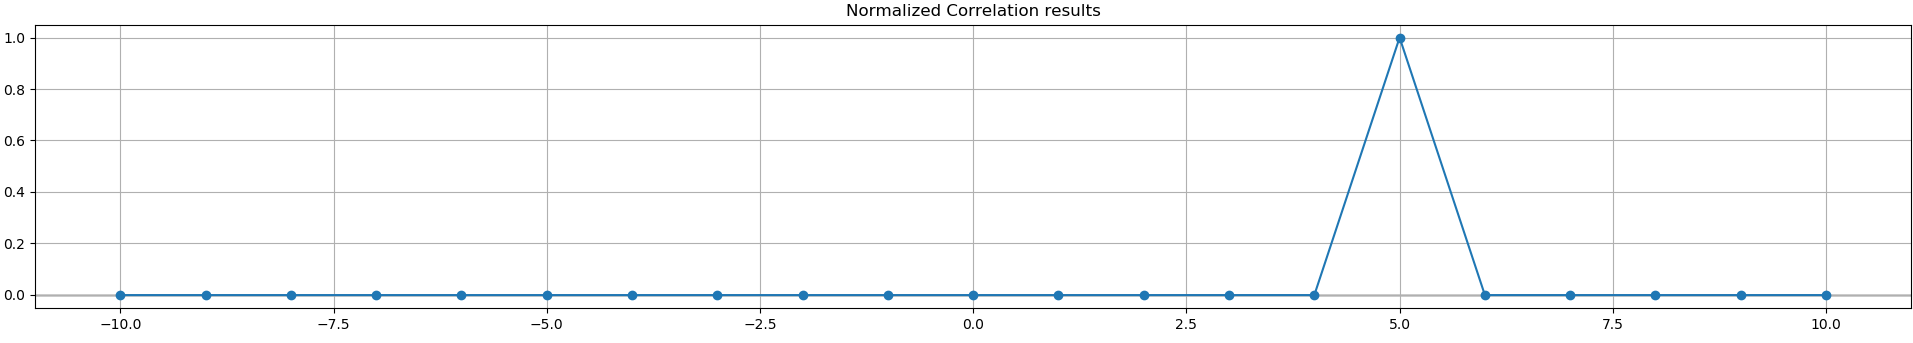
\includegraphics[width=\linewidth]{pythonImplementation/images/correlationSubtractMeamFromResultTrue.PNG}
    \caption[Ergebnis: subtractMeanFromResult = True]{Darstellung des Ergebnis bei \enquote{subtractMeanFromResult = True}. Ausschläge sind besser erkennbar\footnotemark. }
    \label{fig:correlationSubtractMeamFromResultTrue}
\end{figure}
\footnotetext{Quelle: Eigene Darstellung}


\section{Beispiel-Skripte}
Ein Skript welches die Funktion aus diesem Kapitel nutzt ist als Beispiel im Projekt unter \enquote{example\_script\_crosscorrelation.py} abgelegt.\\
Das Skript das im Zuge der Automatisierung verwendet wird, ist im Unterverzeichnis \enquote{crosscorrelation} unter \enquote{automated\_crosscorrelation.py} zu finden.









\chapter{Suche nach Pattern mit Hilfe der Kreuz-Korrelation}
Das Python Skript \enquote{functions\_crosscorrelation\_patternsearch.py} bietet zwei Funktionen an, die verwendet werden können, 
um nach einem gegebenen Pattern in einer Sequenz zu suchen.

\section{Angebotene Funktionen}
Folgende Funktionen werden angeboten:

\subsection{Funktion: getCorrelationDataForPatternSearch}
Mit Hilfe der \enquote{getCorrelationDataForPatternSearch} Funktion kann nach einem Pattern in einer gegebenen Sequenz gesucht werden. Dafür sind folgende Parameter nutzbar:
\begin{description}
    \item[seqA] Die Sequenz in der nach dem Pattern gesucht werden soll. Übergeben in Form eines eindimensionalen Arrays. Die enthaltenen Zahlenwerte müssen in Float konvertierbar sein.
    \item[pattern] Das Pattern nach dem gesucht werden soll. Übergeben in Form eines eindimensionalen Arrays. Die enthaltenen Zahlenwerte müssen in Float konvertierbar sein.
    \item[plotCorrelation] [Default: False] Auf True setzen, wenn die berechnete Kreuz-Korrelation dargestellt werden soll.
\end{description}
Die Funktion gibt die berechnete Kreuz-Korrelation zurück, die in der nächsten Funktion \enquote{extractIndicesFromCorrelationData} verwendet werden kann.
\\
\\
Die Funktion verwendet intern die von NumPy bereitgestellte \enquote{correlate} Funktion. Als Modus wird der in Kapitel~\ref{sec:numpy_correlate_mode} beschriebene Modus \enquote{Valid} genutzt.

\subsection{Funktion: extractIndicesFromCorrelationData}
Die Funktion kann verwendet werden, um die Indizes zu berechnen, an denen das Pattern in der Sequenz auftritt. Dafür muss der Funktion das Ergebnis der \enquote{getCorrelationDataForPatternSearch} Funktion
übergeben werden. Als Rückgabe erhält man die Indizes und der Wert der Korrelation an dieser Stelle.\\
Optional kann ein Schwellwert übergeben werden. Je nachdem wie dieser Schwellwert gewählt ist, werden mehr oder weniger Indizes zurückgegeben. Bei einem hohen Schwellwert wird 
jeweils nur der erste Index zurückgegeben, bei dem das Pattern auftritt. Bei einem niedriger gewählten Schwellwert werden alle Indizes zurückgegeben, an denen das Pattern auftritt. 
Bei einem zu niedrigem Schwellwert werden auch Indizes zurückgegeben, die außerhalb des eigentlichen Patterns liegen. Diese Bereiche sind direkt vor und nach dem Ende des Patterns. Ein zu niedriger Schwellwert kann erkannt werden, wenn der gefundene Bereich größer als das Pattern selbst ist. Durch einen höheren Schwellwert kann dieses \enquote{Auswaschen} oder \enquote{Aufweichen} verhindert werden.

\subsection{Beispiel für die Pattern-Suche}
Vorbedingung: Eine Sequenzen mit 10000 Einträgen. \\
SeqA:
\[ a_{n} =
  \begin{cases}
    1       & \quad \text{wenn } n \text{ enthalten in [1005,1007,1010,6005,6007,6010]}\\
    0  & \quad \text{sonst}
  \end{cases}
\]
Gesuchtes Pattern:
\[
pattern = [1,0,1,0,0,1,0] 
\]
Das Pattern tritt in der gegeben Sequenz zwei Mal auf (an Index 1005 und 6005).
Der Aufruf der \enquote{getCorrelationDataForPatternSearch} Funktion mit dem \enquote{plotCorellation = True} zeigt die in Abbildung~\ref{fig:patternsearchCorrelation} dargestellte Kreuz-Korrelation.

\begin{figure}[H]
  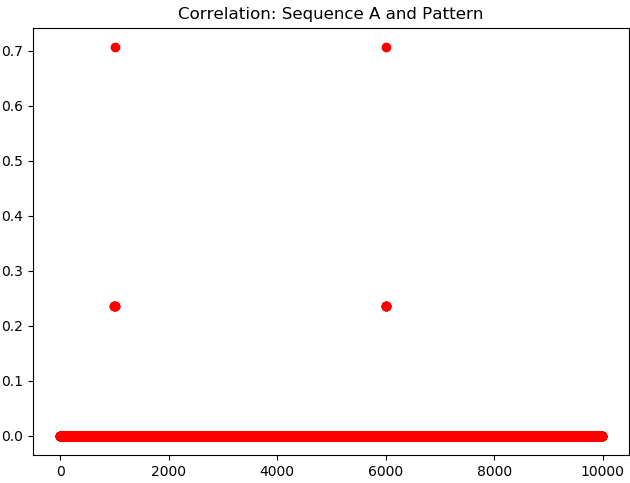
\includegraphics[width=\linewidth]{./images/patternsearchCorrelation.PNG}
  \caption[Patternsuche: Kreuz-Korrelation]{Kreuz-Korrelation der Patternsuche\footnotemark.}
  \label{fig:patternsearchCorrelation}
\end{figure}
\footnotetext{Quelle: Eigene Darstellung}

\begin{samepage}
Mit Hilfe der dargestellten Kreuz-Korrelation kann der Schwellwert für die \enquote{extractIndicesFromCorrelationData} festgelegt werden.
Ein Aufruf mit einem Schwellwert von \enquote{0.3} liefert folgendes Ergebnis: \\
\begin{align*}
   & [6005, 0.70710678], \\
   & [1005, 0.70710678]
\end{align*}

Dabei handelt es sich um die Indizes, an denen das Pattern in der Sequenz beginnt (inklusive den Wert an dieser Stelle). \\
\end{samepage}
\begin{samepage}
Ein Aufruf mit einem Schwellwert von \enquote{0.2} liefert dagegen folgendes Ergebnis: \\
\begin{align*}
  &  [6005, 0.70710678], \\
  & [1005, 0.70710678], \\
  & [6003, 0.23570226], \\
  & [1000, 0.23570226], \\
  & [6007, 0.23570226], \\
  & [6010, 0.23570226], \\
  & [6002, 0.23570226], \\
  & [6000, 0.23570226], \\
  & [1010, 0.23570226], \\
  & [1008, 0.23570226], \\
  & [1007, 0.23570226], \\
  & [1003, 0.23570226], \\
  & [1002, 0.23570226], \\
 & [6008, 0.23570226]
\end{align*}
Darin enthalten sind Indizes im Bereich von 1000 bis 1010 sowie 6000 bis 6010. Die Bereiche sind größer als das Pattern selbst, allerdings ist das Pattern in diesen Bereichen enthalten.
\end{samepage}


\chapter{Automatische Ausführung der Skripte}

\section{Bereitgestellte Skripte}
\textcolor{red}{VS-Code + CMD Anleitung + Darstellung der Ergebnisse von Beispielsequenzen + Logging}

\section{Anleitung zur Ausführung Skripte}

\section{Ablauf der automatisierten Ausführung}

\section{Verbesserungsmöglichkeiten und Erweiterungen}
\textcolor{red}{Multi-Prozess PDF Generierung}




\printbibliography[heading=bibintoc]

\end{document}
